\chapter{Chosen Application Architecture}

After researching available technologies, an architecture to build the pfcrender tool on was selected. The implementation is shown alongside the original requirements in the following graphs, split between functional- (figure \ref{fr}) and non-functional (figure \ref{nfr}) requirements. As before, direct requirements are highlighted in green. Take note that each direct requirement is satisfied or verified through an implementation requirement or test case.

The architecture is discussed in detail in the following sections.

\begin{figure}[p]
	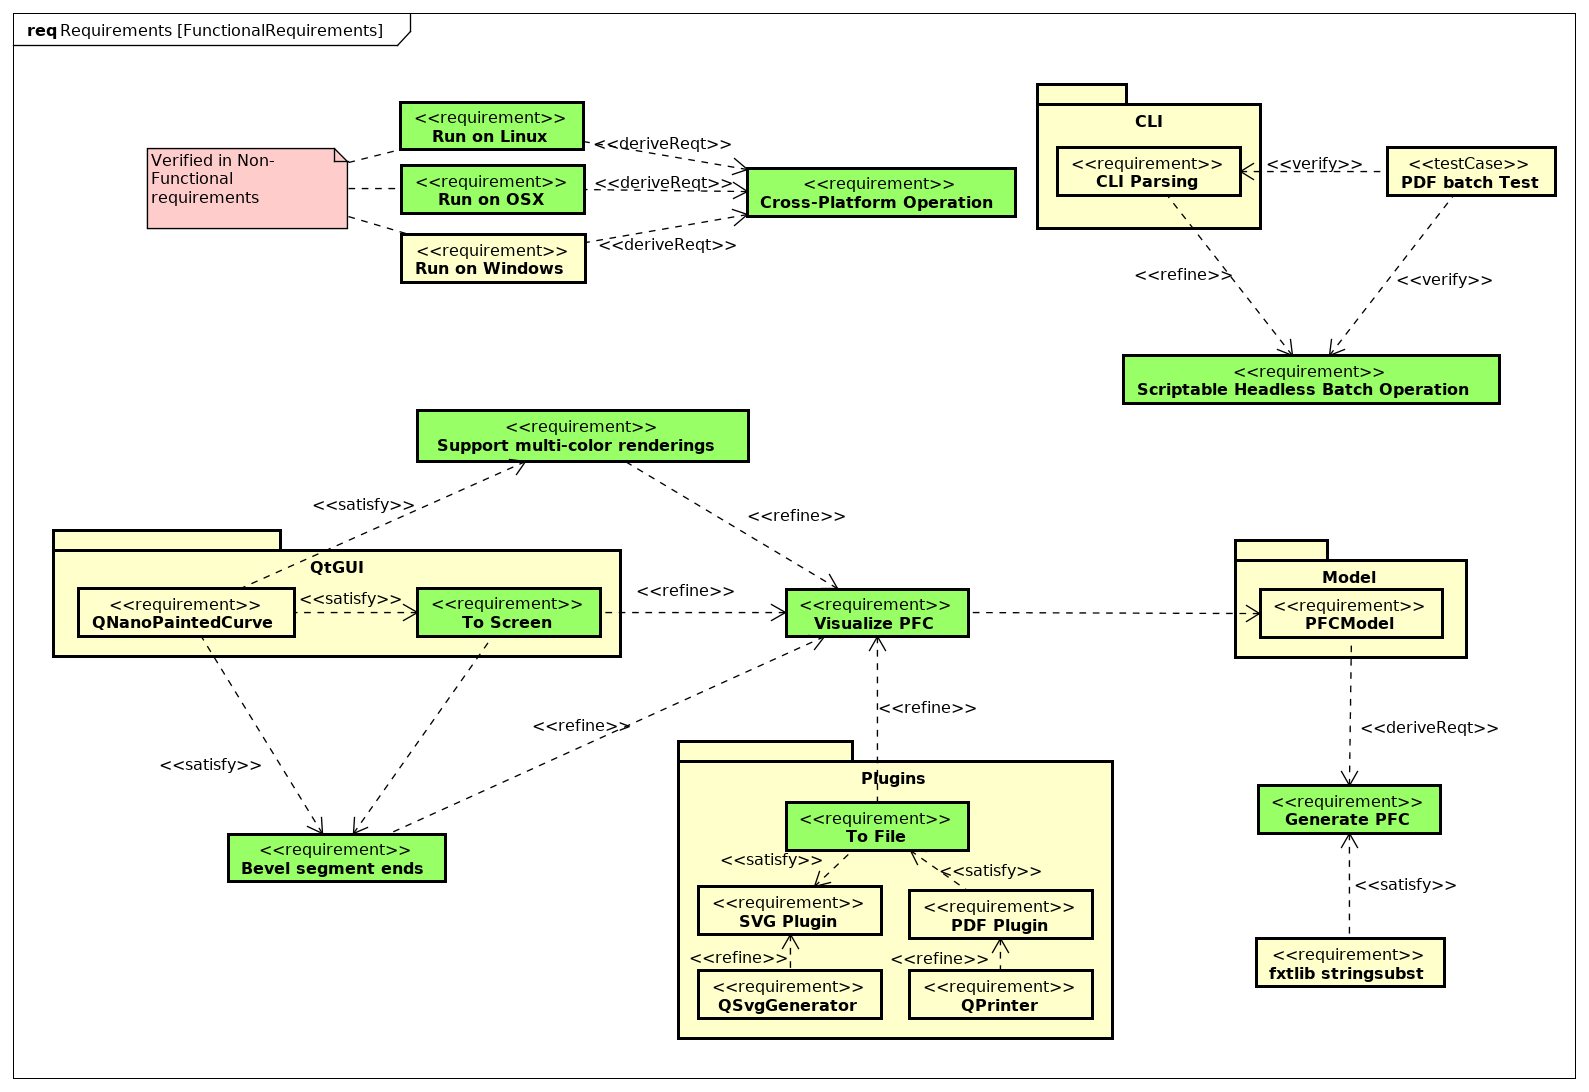
\includegraphics[width=\textwidth]{FunctionalRequirements}
	\caption{Functional requirements}
	\label{fr}
\end{figure}

\begin{figure}[p]
	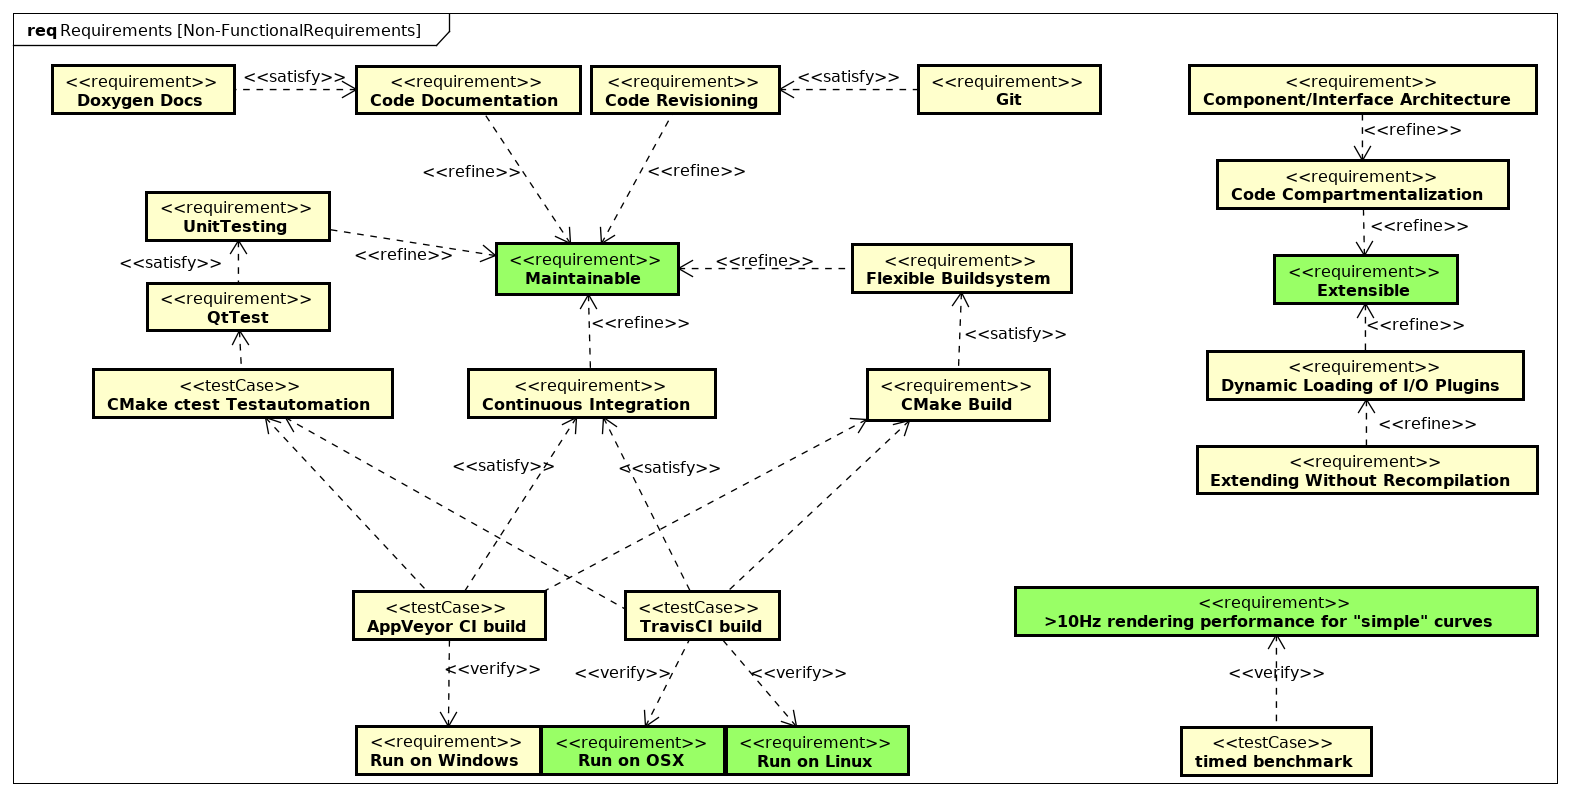
\includegraphics[width=\textwidth]{Non-FunctionalRequirements}
	\caption{Non-functional requirements}
	\label{nfr}
\end{figure}

\section{Functional Requirements}
The main decision to make on the software architecture side was which of the framework libraries discussed in section \ref{sec:res_frameworks} to use.
Selection was driven by three main concerns: extensibility, performance and ease-of-use.

Ultimately, the Qt Framework was chosen for the following reasons:
\begin{itemize}
	\item Platform-independent dynamic library loading abstraction provided, which is useful for implementing a plugin architecture as described in \ref{sec:pluginarch}
	\item Classes provided for exporting e.g. to SVG and PDF
	\item The QtQuick API exposes direct OpenGL access, i.e. rendering performance should not suffer much compared to more light-weight frameworks like \gls{sdl}
	\item Multiple quality-of-life improvements like the QtCreator \gls{ide} with \gls{gui} designer
	\item Included QtTest Unit-Testing Framework
\end{itemize}

Qt provides most of the wanted features in one framework, reducing the amount of necessary dependencies to provide all required functionality. The only additional dependency to Qt introduced to the project is the drawing \gls{api} QNanoPainter(\ref{sec:qnanopainter}), which was introduced as manipulating OpenGL geometry directly proved unwiedly for rendering arcs. 

A description of the Qt provided mechanisms used in this tool follows

\subsection{Dynamic Library Loading}
Windows DLL API mandates symbols callable from outside a library to be prefixed with a macro on export and import. The \gls{msdn}\furl{https://msdn.microsoft.com/en-us/library/3y1sfaz2.aspx} defines it the following way
\begin{lstlisting}
__declspec( dllimport ) declarator  
__declspec( dllexport ) declarator  
\end{lstlisting}

Linux compilers like gcc will not be able to parse this keyword and fail compilation. While it is possible to work around this issue by wrapping the keyword in a preprocessor macro that expands to nothing on Linux, this mechanism is cumbersome to implement.

To get cross-\gls{os} operation without recompiling, use Qt's Library loading mechanism: QPluginLoader OR QLibrary.

This adds an additional step of making Qt's MetaObjectSystem aware of the library but avoids OS-specific switches/preprocessor macros

\subsection{Rendering in Qt}
As stated before, Qt offers two different application programming \gls{api}s. A main difference is in the rendering methode they use:
\begin{description}
	\item [QWidgets] The main API of Qt. It is Java SWING-like and handles GUI design and functionality in C++ using Qt-provided or custom QWidget-derived classes.
	\item [QtQuick] A relatively new (since Qt 4.7) javascript-based declarative language called \gls{qml}, similar to the XML-based JavaFX, is used to define the GUI frontend, while C++ classes in the backend are used for performance intensive calculation. The UI is then rendered in a so-called scenegraph using a platform specific graphics backend like OpenGL or OpenGL ES. Though no formal study of performance differences between both \gls{api}s exists, documentation by the QtCompany\furl{http://doc.qt.io/qt-5/qtquick-performance.html} suggests performance between both models is comparable if some guidelines are followed.
\end{description}

Since the additional model-/view abstraction is very conducive to extensibility, as the declarative nature makes extending the UI easy, QtQuick is selected for the implementation.


The following methods of drawing to these APIs are offered:
\begin{description}
	\item [QPainter] Oldest drawing API of Qt, used in QWidgets. Not directly usable in QtQuick. Offers highest amount of integration to other Qt classes (notably QPrinter and QSVGGenerator)
	\item [QtQuick/QML shape] Placing line segments directly in a \gls{qml} file and loading it to the SceneGraph (creating quadratic bezier curves added in Qt 5.10 (late 2017), too late for this work\furl{https://blog.qt.io/blog/2017/08/10/let-there-be-more-shapes/})
	\item [QtQuick HTML5 canvas] Draws on top of a HTML5 canvas embedded into the qt app.
	\item [QtQuick Item with custom scene graph node] Instantiates a QQuickItem with a custom appearance by setting vertices and material directly\todo{explain what those are}
	\item [QQuickPaintedItem] An adaptation of the QPainter API for the SceneGraph based QtQuick. 
	\item [QNanoPainter] A third party plugin, offering a mixture of QPainter and HTML5 canvas API to draw on an OpenGL framebuffer object to be placed in the QtQuick scene graph. Offers Painter-like productivity with less performance overhead.
\end{description}

The QML and HTML5 APIs were disregarded due to their interpreted and thus slow nature.

This leaves direct QuickItem implementation, QQuickPaintedItem and QNanoPainter-based QuickItem as viable options.

Due to performance measurements\furl{https://www.vikingsoftware.com/qtquick-custom-item-performance/}, a direct implementation was chosen intially (see \ref{somewhere}). The operations performed using this \gls{api} were too inflexible to allow for generation of quadratic bézier curves necessary to implement rounded edges (see \ref{somewhere}), so a higher level \gls{api} was selected.

Further performance benchmarks\furl{http://kgronholm.blogspot.com/2017/12/qt-510-rendering-benchmarks.html} led to preferring QNanoPainter over the built-in QQuickPaintedItem, even though it meant introducing an additional dependency into the project.

It is worth noting, that QPainter \gls{api} was still used for file outputs (see \ref{svg}, \ref{pdf}), where performance is not as critical, due to its integration with other Qt exporter classes.

\section{Non-functional Requirements}

\subsection{Qt Unit Testing Framework}

Qt comes with its own unit-testing framework integrated into QtCreator. The following example is an example test for a fictional Counter class:

\begin{lstlisting}
#include <QtTest>
#include "Counter.h"

class MyTest : public QObject {
    Q_OBJECT

    Counter* ctr;

private slots:
    void initTestCase();

    void do_count();
  //void do_downcount(); // additional test routines

    void cleanupTestCase();
};

void MyTest::initTestCase()
{
	ctr = new Counter(0);
}

void MyTest::cleanupTestCase()
{
    delete ctr;
}

void MyTest::do_count()
{
	ctr->count();
	QVERIFY(ctr->getValue() == 1);
}

QTEST_MAIN(MyTest)
#include "MyTest.moc"
\end{lstlisting}

This builds an executable (main routine provided by the QTEST\_MAIN macro) that runs the given test routines.
It is integrated with QtCreator, which gathers test apps created in this way automatically and can run them from the \gls{gui} and display PASS/FAIL status depending on QVERIFY() and return value.
\begin{figure}[h]
	\todo{qtcreatbild}
\end{figure}

Since it is a standalone executable, it can also be run by other testing environments like CMake's CTest, and can thus be automated and integrated into \gls{ci} builds.

\begin{figure}[h]
	\todo{travis buildlog}
\end{figure}

\subsection{Makefile Generator - CMake}
Though as described in \ref{sec:resMakefileGen} Qt has its own makefile generator with qmake, CMake was selected because of good support in \gls{ci} software, widespread use and thus great documentation, and its built-in CTest Test-Runner, which allows to automatically gather defined unit-tests and run them in a \gls{ci} build. This makes \gls{ci} more informative, as it will not only report failure on changes that break compilation, but also on changes that break functionality for which tests exist. This in turn is a great gain in maintainability of the project and encourages contributors to actually write unit tests, since they don't need to be run manually.

\subsection{Configuration}
It was thus decided to introduce a central store of configuration, that will be accessible to the entire application using the Singleton pattern discussed in section \ref{sec:ston}.

Furthermore, each plugin is required to publish configuration options it wants to this config store and pull its configuration from it.

Since all available commandline options must be known at parsing time for documentation generation and parsing itself, it follows that all plugins must be loaded once on startup to query them for their config options.

While this is not computationally efficient, as not all plugins will necessarily be executed during program runtime and thus get loaded in vain, maintainability outweighs this minor performance issue, as the number of plugins is small. Also, the fact that all plugins must be loaded anyway allows gathering a list of plugins automatically by just loading every library present in the plugins subdirectory instead of maintaining a separate registry of available plugins, e.g. in form of a configuration file, making the program \emph{truly runtime extensible without additional configuration}.

Another problem is gathering options from plugins automatically is possible when building a list of plugins, options exposed by the main application can not be added this easily, as the objects that expose the info structure do not need to exist by the time. So in this instance - for options of the main app - a manual list must be maintained after all. While this difference in behaviour betwenn core and plugins is unfortunate, it is still an improvement over fully manual API documentation.

Due to it supporting our use-case, being easily extensible and not introducing any more dependencies into the project above the already used Qt Framework libraries, the QtCommandLineParser was chosen to provide the main CLI-based interface to the program.
\subsubsection{config stores}
The selected architecture defines an order of precedence of config options:
1. Global options are set from config file is parsed
2. options given on Command line are set 
(3. GUI options can set config settings)

\subsection{Version Control System}
Due to the useful issue tracking feature of github and its extensive third party infrastructure integration with the services like \gls{ci}, git was chosen as \gls{vcs} and github as the central repository provider.

\subsection{CI provider}
Github integration, and free-for-open source service, led to Appveyor being selected as \gls{ci} provider for windows builds, and Travis CI for Linux and MacOS X.

\section{Honorable Mentions}\todo{lol}
\subsection{QtCreator}
\todo{asdf}

\section{Class Hierarchy}
\begin{figure}[p]
	\todo{class diagrams}
\end{figure}
